% This is LLNCS.DOC the documentation file of
% the LaTeX2e class from Springer-Verlag
% for Lecture Notes in Computer Science, version 2.4
\documentclass{llncs}
\usepackage{llncsdoc}
\usepackage{graphicx}
\usepackage{amssymb}
\usepackage[table]{xcolor}
%\usepackage[cp1250]{inputenc} % WH
%\usepackage[polish]{babel}    % WH

% Added for code listing
\usepackage{listings}
\usepackage{caption}

\newcounter{nalg}[chapter] % defines algorithm counter for chapter-level
\renewcommand{\thenalg}{\thechapter .\arabic{nalg}} %defines appearance of the algorithm counter
\DeclareCaptionLabelFormat{algocaption}{Algorithm \thenalg} % defines a new caption label as Algorithm x.y

\lstnewenvironment{algorithm}[1][] %defines the algorithm listing environment
{
    \refstepcounter{nalg} %increments algorithm number
    \captionsetup{labelformat=algocaption,labelsep=colon} %defines the caption setup for: it ises label format as the declared caption label above and makes label and caption text to be separated by a ':'
    \lstset{ %this is the stype
        frame=tB,
        numbers=left,
        numberstyle=\tiny,
        basicstyle=\scriptsize,
        keywordstyle=\color{black}\bfseries\em,
        keywords={,input, output, return, datatype, function, in, if, else, foreach, while, begin, end, done, } %add the keywords you want, or load a language as Rubens explains in his comment above.
        numbers=left,
        xleftmargin=.04\textwidth,
        #1 % this is to add specific settings to an usage of this environment (for instnce, the caption and referable label)
    }
}
{}

\usepackage{url}
\urldef{\mailwhajwp}\path|{xxx,yyy,zzz}@mini.pw.edu.pl|
\newcommand{\keywords}[1]{\par\addvspace\baselineskip
\noindent\keywordname\enspace\ignorespaces#1}
%
\begin{document}


\title{Title}
\author{Wladyslaw Homenda$^{1}$
\and Agnieszka Jastrzebska$^1$
\and Piotr Waszkiewicz$^1$
\and Anna Zawadzka$^1$
}

\authorrunning{W. Homenda, A. Jastrzebska, P. Waszkiewicz, A. Zawadzka}
\institute{$^1$Faculty of Mathematics and Information Science, Warsaw University of Technology\\ul. Koszykowa 75, 00-662 Warsaw, Poland\\
%$^2$Department of Electrical \& Computer Engineering, University of Alberta, \\Edmonton T6R 2G7 AB Canada\\
%\mailwhajwp
}

\titlerunning{xxxxx yyyyyy zzzzzz}
\maketitle

\pagestyle{empty}  % no page numbers, no running headers

\begin{abstract}
In the article we present
\end{abstract}


%-------------------------------------------------------------------
%-------------------------------------------------------------------
%-------------------------------------------------------------------

\section{Introduction}
  \label{sec:Introduction}

The task of pattern recognition is a classical machine learning problem. On the input we pass a training dataset, consisting of labelled patterns belonging to $c$ classes. In the process we expect to form a model that would be able to assign correct labels to new cases (new observations).

It is important to have in mind that patterns in their original form are some sort of signal, for instance images or voice recordings. Due to the fact that the original patterns are often collected using some signal-acquiring devices, we may encounter patterns that do not belong to any of proper classes. An example of such situation may happen, when the device that we use to acquire data has been automatically reset due to power outage and poor default calibration distorts the segmentation process. Another scenario may happen when we collect data in a noisy (out-of-lab) environment and apart from proper patterns there is a lot of unexpected residual elements. The problem with garbage patterns is that we cannot predict their character and therefore we cannot include information about them in the model training process.

The motivation of our study is to provide algorithmic approaches to distinguish proper patterns, that we call \textbf{native patterns} from garbage and erroneous patterns, that we call \textbf{foreign patterns}. The task that we describe we call \textbf{foreign patterns rejection}. The design assumption is to provide methods based on native patterns only. In this way the framework that we propose is truly versatile and it can be adapted to any pattern recognition problem in an uncertain environment, where foreign patterns may appear. 

We propose several classification with foreign elements rejection scenarios based on well-known combinations of machine learning algorithms. The novelty of the contribution presented in this paper is not in the methods that we use, but in what we achieve with them. 
{\color{blue} In particular, the objective of this paper is to discuss ...}

%TODO koniecznie trzeba dodac wiecej opisu novelty/objective, dodamy na koncu jak bedzie calosc artykulu

The proposed methods are applied in a case study of handwritten digits recognition.

The remainder of this paper is organized as follows. Section \ref{sec:Literature Review} presents the background knowledge on foreign elements detection present in the literature. Section \ref{sec:preliminaries} presents the backbone algorithms well-known in the literature that we use to construct our models. Section \ref{sec:Methodology} presents the proposed approach. In Section \ref{sec:Experiments} we discuss a series of experiments based on images of handwritten digits. Lastly, Section \ref{sec:Conclusion} concludes the paper and highlights future research directions.


%-------------------------------------------------------------------
%-------------------------------------------------------------------
%-------------------------------------------------------------------
\section{Literature Review}
  \label{sec:Literature Review}

Data collection and processing is a vital study problem across multiple domains of science. Along with a substantial automation of data acquiring we meet with difficulties that appear due to poor data quality. The research we present in this paper has been motivated by the issue of contaminated datasets, that apart from proper patterns contain garbage.

Let us start our discussion with review of relevant literature positions in machine learning that tackle the issue of contaminated datasets. 

First and foremost let us discuss outlier detection methods. Outliers are native patterns that substantially differ from the remainder of class elements. Detection of outliers is an important domain of machine learning, as many learning methods are very likely to fail, when they process such data. Even though outliers are proper native elements, they are often removed from the training dataset in order to construct a good model. In consequence, it is very likely that appearance of outliers in a testing set would result in their misclassification. However, this is a relatively small price to pay for a model that is well-fitted to model majority of the data. We may distinguish the following groups of methods dealing with outliers:
\begin{itemize}
  \item statistical,
  \item model-based.
\end{itemize}

The first group constitutes of methods based on sample statistics. The second group consists of approaches with a stage of model building. 
 
A very intuitive way to detect outliers is to visualize the data we process, for instance with histograms or box plots. Automating this process typically relies on calculating sample statistics and detecting those observations that differ remarkably from the mean or median. This idea could be briefly summarized by saying that outliers are those elements that fall far from the majority of the data. This straightforward method works fairly well in practice. Model designer is responsible for determining a cutoff threshold to distinguish between outlying and regular observation. There is a wide variety of papers relating to this idea, where various decision rules or tests for outliers are discussed. For instance, we may mention Z-score that is defined as:
\begin{equation}\label{eqn:zscore}
    Z_i = \frac{x_i - \bar{x}}{sd}
\end{equation}
where $\bar{x}$ is sample mean and $sd$ is standard deviation. In \cite{IglewiczHoaglin1993} authors propose a modified Z-score based on median:
\begin{equation}\label{eqn:modifiedzscore}
    MZ_i = \frac{0.6745(x_i - \tilde{x})}{MAD}
\end{equation}
where $\tilde{x}$ is the median and $MAD$ is the median absolute deviation. The authors recommend to set the cutoff point to 3.5. 

It is also worth to mention formal outlier tests: Grubbs' Test, Tietjen-Moore Test, and Generalized ESD Test. Named tests assume that there are no outliers in the data set. However, the alternative hypotheses differ. Grubbs' Test assumes that there is exactly one outlier in the data set, Tietjen-Moore Test assumes that there are exactly $k$ outliers in the data set, while Generalized ESD Test assumes that there are up to $r$ outliers in the data set. In the subsequent steps a simple statistics are computed. It has to be emphasized though that they are also based on simple notions: sample mean, maximal distance from the mean, or standard deviation. 

The second group of outlier detection methods is based on various models. For instance, one may adapt clustering algorithms for outlier detection. A good examples are soft clustering approaches, for instance Gaussian Mixture Models (GMMs) and fuzzy c-means. Those methods express cluster membership as a number from the $[0,1]$ interval. An element, whose dominating membership cannot be easily decided could be regarded as outliers. The limitation of these approaches is that the quality of outliers removal is determined by the quality of internal data structure detection. If an algorithm fails to detect proper clusters, it is likely to reject many proper patterns in process.

Discussion on approaches related to foreign elements rejection should also mention one-class classification methods. Especially, there are two noteworthy examples: centroid-based methods and One-Class Support Vector Machine.

Centroid-based methods rely on distinguishing cluster centres (centroids). Region reserved for proper elements is usually defined by the distance between centre and the furthest proper pattern.

One-Class SVM has been introduced in \cite{ScholkopfWilliamsonSmola1992}. While "regular" SVM algorithm forms hyperplane separating two classes, the One-Class SVM separates data points from the entire feature space. Notably, the One-Class SVM provides a soft decision rules, as there is a $\nu$ parameter determining the fraction for outliers.  

It is worth to emphasize the analogy between outlier detection and foreign elements rejection. However, the motivation for those two problems remains different.

When it comes to the study on foreign elements rejection, there is relatively few papers to review. This issue, in spite of its importance, remains somehow neglected. Among noteworthy studies one may mention rank-based methods, for instance ones described in \cite{BertolamiZimmermannBunke2006,BurgerKessentiniPaquet2011,EladHel-OrKeshet2001,HempstalkFrankWitten2008,SchemeHudginsEnglehart2013,WangCasasent2009}.
In a nutshell, mentioned papers propose to attach confidence scores along with class labels. Rejection occurs when none of native class labels was assigned with a satisfying confidence.

In our paper we assume an approach that in its background resembles more model-based outlier detection techniques than reported in the literature foreign elements rejection schemes. The objective of our study is to form a model that would be able to distinguish between the region reserved for native patterns and the remainder of the feature space. 

%-------------------------------------------------------------------
%-------------------------------------------------------------------
%-------------------------------------------------------------------
\section{Preliminaries - Backbone Algorithms}
  \label{sec:preliminaries}
  
The proposed approach builds upon several existing algorithms. In order to provide a self-contained description of our methods in this section we present backbone literature algorithms applied in our method. In what follows we present the Minimum Volume Enclosing Ellipsoid (MVEE) algorithm and a suite of 3 classification methods: Random Forests (RF), Support Vector Machines (SVM), and K-Nearest Neighbors algorithm (K-NN). Listed methods are employed in various configurations to native elements classification with foreign elements rejection. Our approach, based on those algorithms, is discussed in Section \ref{sec:Methodology}.

%-------------------------------------------------------------------
%-------------------------------------------------------------------
\subsection{Ellipsoids for Foreign Elements Rejection}

%description of the idea of geometrical rejection
%issues: location, size, parameters of those figures

% Links used in this description
% Link: http://geomalgorithms.com/a08-_containers.html
% http://people.orie.cornell.edu/miketodd/TYKhach.pdf
Both native and foreign elements consist of certain number of features extracted from scanned symbols. Such data can easily be represented in multidimensional space where dimension degree equals number of those features. What's more, if it turned out that the sets of those points representing symbols, each forms a tight cluster in space, it might be possible to find their respective minimal enclosing boxes.

In computational geometry, the smallest enclosing box problem is that of finding the oriented minimum bounding box enclosing a set of points. As opposed to convex hull, which is the most accurate point set container with smallest volume, bounding boxes are far less complex. In many cases, when there's a need for computing convex hull and testing inclusions of other points, an approximation of such hull can be used, which helps to reduce time needed for computations, since most of alternative methods have lower construction and inclusion-testing complexities. Some of such approaches include using figures like hypercubes, diamonds, spheres or ellipsoids to successfully enclose given set of points.

When comparing highlights and drawbacks of each method, from computational complexity, ease of testing point inclusion and algorithm implementation point of view, ellipsoids seem to be a reasonable choice. Constructed ellipsoid is superior to the minimal cuboid in many ways. It is unique, better approximation of the object it contains and if $E(S)$ is the bounding ellipsoid for a point set $S$ with convex hull $C(S)$ in dimension \textit{d}, then:
\[ \frac{1}{d}E(S) \subseteq C(S) \subseteq E(S) \]
where scaling is with respect to the center of $E(S)$.

Adaptation of the smallest enclosing box problem to foreign elements rejection, or native elements identification, seems to be a very natural approach. The justification is fairly simple: if we enclose elements belonging to native classes, using for instance ellipsoids, formed geometrical model will discriminate a region of features space reserved for native patterns between a region where we may encounter foreign patterns. With this premise in mind, let us present a detailed description of the MVEE algorithm.

%-------------------------------------------------------------------
\subsubsection{MVEE}

% Links used:
% http://citeseerx.ist.psu.edu/viewdoc/download;jsessionid=3A12C2006473A250D78C45B99B0BB3FA?doi=10.1.1.116.7691&rep=rep1&type=pdf
% http://www.mathworks.com/matlabcentral/fileexchange/9542-minimum-volume-enclosing-ellipsoid/content/MinVolEllipse.m
% http://stackoverflow.com/questions/1768197/bounding-ellipse/1768440#1768440
% http://stackoverflow.com/questions/14016898/port-matlab-bounding-ellipsoid-code-to-python

problem is solved by several known algorithms that can be categorized as first-order, second-order interior-point or combination of the two. For small dimensions \textit{d}, the MVEE problem can be solved in \textit{O($d^{O(d)}$m)} operations using randomized or deterministic algorithms\cite{MVEEMichaelTodd2005}. In this paper the algorithm based on Khachiyan solution is used.

\noindent An ellipsoid in center form is given by \[ E = \{x \in \mathbb{R}^{n} | (x - c)^{T}A(x-c) \le 1\} \] where $c \in \mathbb{R}^{n}$ is the center of the ellipse E and $ A \in \mathbb{S}^{n}_{++}$ Points lying inside the ellipse satisfy \[ (x_{i} - c)^{T}A(x_{i} - c) \le 1 + acceptance \] where acceptance parameter defines the error margin in determining point belonging to ellipsoid. It can be imagined as testing point inclusion on enlarged ellipsoid.

However, presented equation, is not a convex optimization problem and it has to be changed. It turns out that even then, the solution is not easily obtainable so the dual problem has to be found. For more precise and in depth solution description see \cite{MVEEMichaelTodd2005}. The main problem, when using ellipsoids as identifiers, lies in constructing them. Two main factors that decide about identification effectiveness are tolerance and acceptance parameters. Tolerance can be viewed as a threshold for ellipsoid construction accuracy. The lower the parameter is, the better minimal volume ellipsoid is created. On the other hand, even with good training set, there's a risk of including native elements that lie outside of created ellipsoid. To prevent such unwanted behaviour acceptance has been introduced. It defines threshold for point rejection for those points that lie outside of created figure.  

%{\color{red}Na razie prosze nie zmieniac struktury rozdzialu 3. Dostosujemy ten rozdzial do pozostalej czesci pracy.}

\noindent The pseudocode for the MVEE algorithm used in this paper is as follows:
% Code taken from:
% http://www.mathworks.com/matlabcentral/fileexchange/9542-minimum-volume-enclosing-ellipsoid/content/MinVolEllipse.m
% http://stackoverflow.com/questions/14016898/port-matlab-bounding-ellipsoid-code-to-python
\begin{algorithm}[mathescape=true, caption={MVEE}, label={alg1}]
input:
    $\textbf{P}$ - row-ordered matrix of m n-dimensional points
    $\textbf{tolerance}$ - solution error value with respect to optimal value

output:
    $\textbf{c}$ - center point of found ellipsoid
    $\textbf{A}$ - matrix %TODO Add description

begin
    N $\leftarrow$ number of points in P
    d $\leftarrow$ number of dimensions for points in P

    Q $\leftarrow
    \pmatrix{%
        P_{1,1} & P_{1,2} & \dots & P_{1, n} & 1 \cr
        P_{2,1} & P_{2,2} & \dots & P_{2, n} & 1 \cr
        \vdots & \vdots & \ddots & \vdots & \vdots \cr
        P_{m,1} & P_{m,2} & \dots & P_{m, n} & 1 \cr
    }$

    error $\leftarrow$ 1

    u $\leftarrow [\frac{1}{N}, \frac{1}{N}, \dots, \frac{1}{N}]$, |u| = N

    while error > tolerance
        X $\leftarrow Q * \pmatrix{%
            u_{1} & 0 & \dots & 0 \cr
            0 & u_{2} & \dots & 0 \cr
            \vdots & \vdots & \ddots & \vdots \cr
            0 & 0 & \dots & u_{n} \cr
        } * Q^{T}$

        M $\leftarrow$ diag($Q^{T} * X^{-1} * Q$)

        jdx $\leftarrow$ $M_{j} : \forall_{0 \le i \le |M|} M_{j} \ge M_{i}$

        step_size $\leftarrow$ $\frac{M[jdx] - d - 1.0}{(d+1) * (M[jdx] - 1.0)}$

        new_u $\leftarrow$ (1 - step_size) * u

        new_u[jdx] $\leftarrow$ new_u[jdx] + step_size

        error $\leftarrow ||new_u - u|| $

        u $\leftarrow$ new_u
    done

    c $\leftarrow$ u * P
    A $\leftarrow \frac{(P^{T} * \pmatrix{%
            u_{1} & 0 & \dots & 0 \cr
            0 & u_{2} & \dots & 0 \cr
            \vdots & \vdots & \ddots & \vdots \cr
            0 & 0 & \dots & u_{n} \cr
        } * P - c^{T} * c)^{-1}}{d}$
end
\end{algorithm}

{\color{blue}For a detailed pseudo-code of the MVEE algorithm one may consult [xx] and [yy]. - prosze dodac uzyte odwolania}

%-------------------------------------------------------------------
%-------------------------------------------------------------------
\subsection{Native Elements Classification}

The task of native elements classification relies on forming a model based on a labelled training dataset that assigns proper class labels to new problem instances. In a conventional scenario the training dataset consists of $m$ instances of $n$-dimensional feature vectors. Feature vectors are numerical descriptors of actual patterns. There is a multitude of classification algorithms, among which we have selected 3 different ones that are applied in our methods. It is necessary to emphasize that if someone would like to adapt our method to their own domain, those algorithms could be substituted with some other classification tools that may be more efficient in that domain. Without further ado let us move towards a brief description of the methods that we apply in our study.

%-------------------------------------------------------------------
\subsubsection{Support Vector Machines}

% Used links:
% http://scikit-learn.org/stable/modules/svm.html#svm-kernels
are a set of supervised learning methods used for classification, regression and outliers detection. The SVM algorithm relies on a construction of hyperplane with a maximal margin that is separating instances of two classes, \cite{CortesVapnik1995}. SVMs are effective in high dimensional spaces, memory efficient and quite versatile with many kernel functions that can be specified for the decision function. Although in some cases, where number of features is much greater than the number of samples, this method can give poor results, and is not cost-efficient when calculating probability estimates, it is well suited for problem presented in this paper. Given a set of training examples, each marked for belonging to one of two categories, an SVM training algorithm builds a model that assigns new examples into one category or the other. For multi-class classification "one-against-one" approach is used. For \textit{n} classes \textit{n} * (\textit{n} - 1) / 2 classifiers are constructed, each trains data from two different classes. The order for classes 0 to \textit{n} is "0 vs 1", "0 vs 2", \dots "0 vs \textit{n}", "1 vs 2", \dots "\textit{n} - 1 vs \textit{n}".

%-------------------------------------------------------------------
\subsubsection{Random Forests}

is a popular ensemble method. The main principle behind ensemble methods, in general, is that a group of "weak learners" can come together to form a "strong learner". In the Random Forest algorithm the weak learners are decision trees, which are used to predict the membership of objects in the classes. For vector of independent variables representing one object they calculate the value of the class the object belongs to by dividing value space into two or more subspaces. More precisely, an input data is entered at the top of the tree and as it traverses down the tree the data gets bucketed into smaller and smaller sets. In this method a large number of classification trees is generated. To grow each tree a random selection with replacement is made from the examples in the training set $D$. Those subsets $D_{k}$ are called bootstrap training sets. At each node $m$ variables are selected at random out of the set of input variables and the best split on these $m$ is used to split the node. After a relatively large number of trees is generated, they vote for the most popular class. Random Forests join few important benefits: (a) they are relatively prone to the influence of outliers, (b) they have an embedded ability of feature selection, (c) they are prone to missing values, and (d) they are prone to overfitting, \cite{Breiman2001}. 




%-------------------------------------------------------------------
\subsubsection{K-Nearest Neighbors}

is an example of a "lazy classifier", where the entire training dataset is a model. There is no typical model building phase, hence the name. Class membership is determined based on class labels encountered in K closest observations in the training dataset, \cite{Altman1992}. In a typical application, the only choices the model designer has to make are selection of K and distance metrics. Both are often extracted with a help of a supervised learning procedures.
%TODO te opisy mozna rozszerzyc - czy dodac to potem zdecydujemy

%-------------------------------------------------------------------
%-------------------------------------------------------------------
%-------------------------------------------------------------------
\section{Methodology}
  \label{sec:Methodology}
  
There are two approaches used to determine whether an object is rejected (classified as foreign). First one assumes the use of classification methods, which originally were not designed for elements rejection. The second approach involves using classifiers as the only classification tool, whereas rejecting is realized by ellipsoids. In this section let us present our methods for foreign elements rejection.

%-------------------------------------------------------------------
%-------------------------------------------------------------------
\subsection{Internal Rejecting}
  \label{subsec:InternalRejecting}

Contrary to ellipsoids, where rejecting points and identifying them as foreign elements is straightforward - such points lie outside of constructed figure, classifiers are not designed for outliers detection. Rejection has to be simulated by constructing specific rules for those tools.

First attempt at creating rejecting binary classifiers based on assumption that foreign elements are not very similar to native ones. Such situation would be easy to recognize by creating one-versus-rest classification schema, where point would be either assigned to a particular class, or considered to be outside of it. By creating one such classifier for every existing class, point would be rejected after falling to "outside group" every time. There are several problems with this conception, though. First of all, what happens when more than one classifier accepts point as native, e.g. should such element be considered foreign? In this paper such point was classified as an element from the class that was lower in the rank, in other words computations were stopped as soon as first classifier recognized element as native.

Second approach required creating $\frac{n * (n-1)}{2}$ classifiers (where n is the number of all native classes), one for each unique pair of classes. In this situation each element classification would end up with result vector containing number of times when tested point was recognized as native for each class. Rejection would be based on too small differences between two best classes. Unfortunately during tests it turned out that differences were often too small even for native elements and this kind of classifier didn't work as expected.

The third way of dealing with classifiers rejection would be to accept only those elements which manage to score enough points in corresponding result vector. The threshold should be arbitrary chosen to minimize native element rejection. This method could be used along with second one and possibly enhance it effectiveness.

{\color{blue} Pewnie tez nalezy dodac schemat - pseudokod? opisujacy internal rejecting.}

%-------------------------------------------------------------------
%-------------------------------------------------------------------
\subsection{External Global and Local Rejecting}
  \label{subsec:GlobalLocalRejecting}

Whereas ellipsoids are good identifiers, they lack in element classification quality. This is caused by ellipsoids sometimes overlapping each other, which results in points belonging to both classes at the same time. Although this can be solved by calculating distance between those elements and each ellipsoid centre, or taking value of ellipsoid-inclusion equation as a classification measure, tests have proven that such approaches are more prone to errors than other classifiers mentioned in this paper. Taking into considerations both strengths and weaknesses of classifiers and identifiers, the combined solution has been prepared that combines both tools, making use of their advantages.

Classifiers have high success rate but cannot distinguish between foreign elements and native ones. Contrary to that, ellipsoids tend to be better at rejecting outliers which makes them good at identifying points that should not be classified. The natural way of dealing with that problem would be to use ellipsoids as first-entry identifier that purifies input set by removing foreigners. The result of such rejection would be sent to the chosen classifier that would classify remaining native elements. Schema of this method is presented on Figure ~\ref{fig:nativeforeignpatternsClassification1}


\begin{figure}[!h]
  \centering
  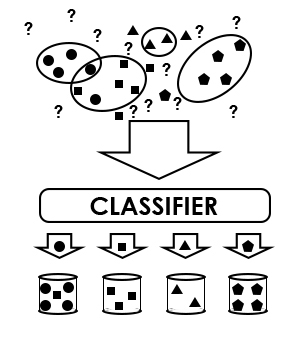
\includegraphics[width=0.7\textwidth]{_Figures/Classification1.jpg}
%  \includegraphics[width=0.7\textwidth]{_Figures/}
  \caption{Ellipsoids as identifiers reject foreign elements and send the rest to classifier for classification}
\label{fig:nativeforeignpatternsClassification1}
\end{figure}

Another way of using ellipsoids as identifiers is to treat them as correctors. That means there's no need to remove foreign elements from the set before classification, as rejection is done later. After all elements have been classified, identification for each class is done by using class-corresponding ellipsoid. There's a possibility that some foreign elements will be assigned to a class with a corresponding ellipsoid that will reject them. This is somewhat different from previous approach because elements can be rejected even if there is an ellipsoid that would pass inclusion test. The schema can be seen on Figure ~\ref{fig:nativeforeignpatternsClassification2}

\begin{figure}[!h]
	\centering
	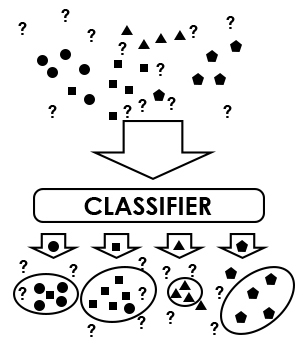
\includegraphics[width=0.7\textwidth]{_Figures/Classification2.jpg}
	%  \includegraphics[width=0.7\textwidth]{_Figures/}
	\caption{Ellipsoids as correctors. Classifiers try to classify foreign elements that will be rejected later}
	\label{fig:nativeforeignpatternsClassification2}
\end{figure}


%-------------------------------------------------------------------
%-------------------------------------------------------------------
\subsection{Quality Evaluation}

In order to evaluate the quality of proposed methods the patterns from the following groups are counted:
\begin{itemize}
\item CC  (Correctly Classified) - correctly classified patterns, i.e. native patterns classified as native ones with the correct class,
\item TP  (True Positives) - native patterns classified as native (no matter, into which native class),
\item FN  (False Negatives) - native patterns incorrectly classified as foreign,
\item FP  (False Positives) - foreign patterns incorrectly classified as native,
\item TN  (True Negatives) - foreign patterns correctly classified as foreign.
\end{itemize}
These numbers are then used to form measures reflecting specific aspects of classification and rejection, cf. Table~\ref{tab:measures}. Notions that we use are well-known in the domain of pattern recognition. We have included a detailed description of those measures in our previous paper \cite{HomendaICAART2015}.
\begin{table}[!htbp]
\centering
\caption{Quality measures for classification and rejection}
{\small
\begin{tabular}{rclrcl}
  $\textnormal{Native Precision}$ &$=$& $\displaystyle\frac{\textnormal{TP}}{\textnormal{TP+FP}}$ & 
  $\textnormal{Accuracy}$ &$=$& $\displaystyle\frac{\textnormal{TP+TN}}{\textnormal{TP+FN+FP+TN}}$ \\
  &&&&&\\
  $\textnormal{Foreign Precision}$ &$=$& $\displaystyle\frac{\textnormal{TN}}{\textnormal{TN+FN}}$ &
  $\textnormal{Strict Accuracy}$ &$=$& $\displaystyle\frac{\textnormal{CC+TN}}{\textnormal{TP+FN+FP+TN}}$ \\
  &&&&&\\
  $\textnormal{Native Sensitivity}$ &$=$& $\displaystyle\frac{\textnormal{TP}}{\textnormal{TP+FN}}$ &
  $\textnormal{Fine Accuracy}$ &$=$& $\displaystyle\frac{\textnormal{CC}}{\textnormal{TP}}$ \\
  &&&&&\\
  $\textnormal{Foreign Sensitivity}$ &$=$& $\displaystyle\frac{\textnormal{TN}}{\textnormal{TN+FP}}$ &
  $\hspace{18pt}\textnormal{Strict Native Senssitivity}$ &$=$& $\displaystyle\frac{\textnormal{CC}}{\textnormal{TP+FN}}$\\
  &&&&&\\
  \multicolumn{6}{c}{$\textnormal{F--measure}=2\cdot\displaystyle\frac{\textnormal{Precision}\cdot\textnormal{Sensitivity}}{\textnormal{Precision}+\textnormal{Sensitivity}}$}\\
\end{tabular}
}
\label{tab:measures}
\end{table}

\begin{itemize}
  \item \emph{Strict Accuracy} measures classifier's performance. It is the ratio of the number of all \emph{correctly classified} patterns to the number of all patterns being processed.
  \item \emph{Accuracy} is a "softer" characteristic derived from the Strict Accuracy. Accuracy describes the ability to distinguish between native and foreign patterns. The difference is that we do not require that the native patterns are labelled with their proper class label.
  \item \emph{Native Precision} is the ratio of the number of not rejected native patterns to the number of all not rejected patterns (i.e. all not rejected native and foreign ones). The higher the value of this measure, the better ability to distinguish foreign elements from native ones. Native Precision does not evaluate how effective identification of native elements is.
  \item \emph{Native Sensitivity} is the ratio of the number of not rejected native patterns to all native ones. The higher the value of Native Sensitivity, the more effective identification of native elements. Unlike the Native Precision, this measure does not evaluate the effectiveness of separation between native and foreign elements.
  \item \emph{Strict Native Sensitivity} takes only correctly classified native patterns and does not consider native patterns, which are not rejected and assigned to incorrect classes, unlike Native Sensitivity, where all not rejected native patterns are taken into account.
  \item \emph{Fine Accuracy} is the ratio of the number of native patterns classified to correct classes, i.e. assigned to their respective classes, to the number of all native patterns not rejected. This measure conveys how precise is correct classification of not rejected patterns.
  \item \emph{Foreign Precision} corresponds to Native Precision.
  \item \emph{Foreign Sensitivity} corresponds to Native Sensitivity.
  \item  Precision and Sensitivity are complementary and there exists yet another characteristic that combines them: the \textit{F--measure}. It is there to express the balance between precision and sensitivity since these two measures affect each other. Increasing sensitivity can cause a~drop in precision since, along with correctly classified elements, there might be more incorrectly classified.
\end{itemize}


%-------------------------------------------------------------------
%-------------------------------------------------------------------
%-------------------------------------------------------------------
\section{Experiments}
  \label{sec:Experiments}

In this section we move towards description of a series of experiments where we apply rejection strategies discussed theoretically in Sections \ref{subsec:InternalRejecting} and \ref{subsec:GlobalLocalRejecting}. In what follows we describe the datasets, experiments' settings and the results. 

%-------------------------------------------------------------------
%-------------------------------------------------------------------
\subsection{Datasets}

The Experiments' section is devoted to a study of handwritten digits recognition. 

Foreign patterns are usually of unexpected shapes and origin. In this study as foreign patterns we assume a dataset of handwritten letters from the Latin alphabet. The justification to assume such foreign dataset for testing purposes is that appearance of other real symbols, not belonging to any proper class, is a common issue in a character recognition problem. 

We would like to stress again, that foreign patterns do not participate in model building phase. The entire scheme is based on native patterns only. Handwritten letters are used only for rejection mechanisms quality evaluation.

Samples of processed patterns are displayed in Figure \ref{fig:nativeforeignpatterns}.

\begin{figure}[!htbp]
  \centering
  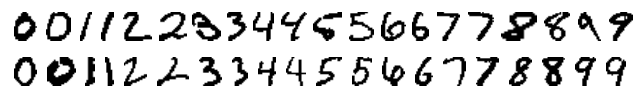
\includegraphics[width=0.49\textwidth]{_Figures/natives}\\
  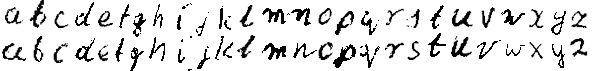
\includegraphics[width=0.7\textwidth]{_Figures/foreigns}
  \caption{Top: samples of handwritten digits - native patterns in our study. Bottom: samples of handwritten letters - foreign patterns in our study.}
\label{fig:nativeforeignpatterns}
\end{figure}

The training dataset was made of 10,000 handwritten digits with approximately 1,000 observations in each class taken from publicly available MNIST database, \cite{LeCunCortesBurges}. We split each class in proportion 7:3 and in a process we got two sets. First one was made of 6,999 observations and we used it for training purposes. The second set was the test set and it contained 3,001 observations. 
We have constructed the foreign dataset by ourselves and it contained 26,000 handwritten letters, 1,000 letters in each class. xxx different people have had participated in the creation of this dataset.

All patterns were normalized and feature vectors comprising of 106 numerical features were created. Feature vectors described not only but also: projections, histograms of projections, transitions, offsets, minimum/maximum values, raw moments, central moments, etc. Subsequently, we have applied best first search method to select relevant features out of the entire feature set. 

Best first search is one of popular wrapper feature selection methods. Wrapper methods select multiple subsets of features, for all those subsets they train a classifier (in general: a model) and they select this subset for which numerical quality was the best. In our particular case as quality evaluator we used a 10-class SVM. A commonly known advantage of wrapper feature selection methods is that the subsets they select usually provide satisfying performance. The disadvantage is their computational complexity. The best first search for the optimal feature subset has been performed using FSelector R package, \cite{Romanski}. The final feature vector contained 24 features. We considered features standardization but the training data is suffitiently consistent (there is no outliers), so we normalized those features to bring all values into the range [0,1]:
\begin{equation}\label{eqn:normalization}
    X'_{i,j} = \frac{X_{i,j} - Min_{j}}{Max_{j}-Min_{j}}
\end{equation}
where $X_{i,j}$ is the value of $j^{th}$ feature in $i^{th}$ observation, $Min_{j}$ and $Max_{j}$ are respectively the minimum and maxium value of $j^{th}$ feature.


%-------------------------------------------------------------------
%-------------------------------------------------------------------
\subsection{Experimental Settings}

Solution presented in this paper has been prepared in form of computer programs, written in Python programming language, using well known scientific libraries - NumPy\footnote{NumPy website: http://www.numpy.org/}, Scikit\footnote{Scikit website: http://scikit-learn.org/stable/}. Implementations of classifiers described in this article have been imported from Scikit library \cite{ScikitSVM,ScikitRF,ScikitKNN}.\\

The MVEE algorithm, available as MATLAB code\footnote{http://www.mathworks.com/matlabcentral/fileexchange/9542-minimum-volume-enclosing-ellipsoid/content/MinVolEllipse.m} has been rewritten in Python language, using NumPy library for matrix representation and operations. Several tests have been performed in order to find best suited method parameters for both classifiers and identifiers. For finding those values the Grid Search\footnote{Link to Python implementation: http://scikit-learn.org/stable/modules/grid\_search.html} has been used for SVM and Random Forests. Ellipsoids and KNN methods had their values assigned manually. 

\subsubsection{MVEE method parameters}
Each ellipsoid was created and used with two parameters: tolerance and acceptance. The tolerance argument was used during creation phase, as "accuracy measurement". Lower value means that created enclosing figure is more fitted to the construction set. Acceptance parameter defines how far can point lie outside the ellipsoid to still be identified as belonging to it. In other words, it treats enclosing ellipsoid as being bigger than it really is.
Parameters tests involved computing effectiveness of MVEE algorithm for certain tolerance and acceptance values. We tested values from such ranges:
\begin{itemize}
	\item tolerance = [0.5, 0.2, 0.1, 0.01]
	\item accuracy = [0.1, 0.01, 0.001, 0.0005]
\end{itemize} 
The results revealed that for given training and test sets the best parameter combination was tolerance=0.001 and accuracy=0.01 and those values were used in final, combined method described later in this document.

\subsubsection{SVM method parameters}
SVM method available in Scikit package offers some built-in kernels that were used during computations: rbf and polynomial. Additionally, there are two more parameters that were tested: C (described as penalty parameter C of the error term), and $\gamma$ (known as kernel coefficient). Values that were tested:
\begin{itemize}
	\item kernel = ['rbf', 'poly']
	\item C = [1, 2, 4, 5, 16]
	\item $\gamma = [2^{-1}, 2^{-2}, 2^{-3}, 0,00025]$
\end{itemize}
The best found combination of those parameters used rbf kernel along with C=8 and $\gamma = 2^{-1}$ values.

\subsubsection{Random Forests method parameters}
RandomForestClassifier method from Scikit library bulids forest of decision trees. The parameter given to the method is the number of trees in the forest. Computations were made using the following values: 1, 2, 3, 5, 10, 20, 30, 40, 50, 60, 70, 80, 90, 100, 110, 120, 130, 140, 150. The best number of trees to build the forest is 100.

\subsubsection{KNN method parameters}
The method in Scikit package used to create K-Nearest Neighbors classifier is KNeighborsClassifier. We tested values of K (number of neighbors) such as: 1, 2, 3, 4, 5, 10, 20, 30, 40, 50. The best found value of K is 4. There is also one parameter - metric, but we use default value, which is standard Euclidean metric.

% By?y przeprowadzone testy ACC/TOL i w spos�b empiryczny wybrane warto?ci

%-------------------------------------------------------------------
%-------------------------------------------------------------------
\subsection{Concept of Classification with Rejection}
  \label{subsec:ClassificationAndRejection}

To determine effectiveness of parameter values for each method, confusion matrix has been calculated. Each row of this matrix represents information about points distribution for elementes from certain class. Numbers in each column hold information about quantity of points that were classified as belonging to corresponding class.


\begin{table*}[h]
\centering
\caption{Confusion table for MVEE algoritm with tolerance=0.2 acceptance=0.1 on training set}
%\vspace{3pt}
\setlength{\tabcolsep}{3pt}
\renewcommand{\arraystretch}{1}

{\small
\begin{tabular}{|c||r|r|r|r|r|r|r|r|r|r|r|}
\hline
 \hspace{15pt} & $0\;\;\;$ & $1\;\;\;$ & $2\;\;\;$ & $3\;\;\;$ & $4\;\;\;$ & $5\;\;\;$ & $6\;\;\;$ & $7\;\;\;$ & $8\;\;\;$ & $9\;\;\;$ & $f$ \\
\hline\hline
  0 & 213 & 4 &   &   &   &   & 2 &   & 17 &   & 58\\
\hline
  1 &  & 259 & 1 &   &   &   &   &   &   &   & 81\\
\hline
  2 &  &   & 227 &   &   &   &   &   &   &   & 83\\
\hline
  3 &  &   &   & 206 &   & 4 &   & 2 & 2 &   & 89\\
\hline
  4 &  &   &   &   & 202 &   &   & 2 & 1 & 2 & 88\\
\hline
  5 &  &   &   & 5 & 1 & 189 &   &   & 2 &   & 71\\
\hline
  6 &  & 1 &   &   &   &   & 219 &   & 1 &   & 67\\
\hline
  7 &  &   & 1 &   & 1 &   &   & 243 &   & 1 & 63\\
\hline
  8 & 1 &   &   &   & 1 &   &   &   & 213 &   & 78\\
\hline
  9 &  &   &   &   & 6 & 1 &   & 6 & 2 & 230 & 58\\
\hline
$f$ & 66 & 20 & 48 &   & 110  & 16 & 54 & 1 & 126 & 15 & 25927\\
\hline
\end{tabular}
}

%\vspace{12pt}
\label{tab:CofusionTable}
\end{table*}

Calculations and measurements included in "Quality Evaluation" section were based on confusion matrixes. Information gathered from them will be used in the following sections of this document. The most interesting aspects of it consist of classification quality, rejection quality and rejection impact on classification quality. Those issues are the main and most important part of problem described in this paper.

%-------------------------------------------------------------------
%-------------------------------------------------------------------
\subsection{Classification Quality}

%ideally rejection improves classification by rejecting those element that would have been incorrectly classified

\begin{table}[h]
\centering
\caption{Results for classification with rejection on train and test sets of native patterns in comparison with classification results without rejection mechanism. RF - results for random forest, SVM - results for Support Vector Machines, .... \color{red}W ponizszej tabelce beda dane dotyczace odrzucania tylko na natives za pomoc� elipsoid i na dwoch poziomach (global i local). Czy jest sens dla train set? Czy nie bedzie 100\%? Na poziomie local chyba nie bedzie 100\%, dlatego jest sens. {\color{blue}Jako ostatnie dodane jest internal rejecting - czy dajemy te wyniki?} }
%\vspace{3pt}
\setlength{\tabcolsep}{6pt}
\renewcommand{\arraystretch}{1}
\begin{tabular}{|r||ccc||ccc||}
\hline
& \multicolumn{3}{c||}{no rejection} & \multicolumn{3}{c||}{with rejection}  \\
\hline
  Basic Classifier & RF & SVM & KNN &  RF & SVM & KNN  \\
\hline
  \multicolumn{7}{|c||}{{\color{red}external global rejection}} \\
  \hline
  Data Set & \multicolumn{6}{c||}{Native Patterns, Train/Test?? Set} \\
\hline
Fine Accuracy                & $$ & $$ & $$ & $$ & $0.978$ & $$ \\
Strict Native Sensitivity    & $$ & $$ & $$ & $$ & $$ & $$ \\
Native Sensitivity           & $$ & $$ & $$ & $$ & $$ & $$ \\
\hline
  \multicolumn{7}{|c||}{{\color{red}external local rejection}} \\
\hline
  Data Set & \multicolumn{6}{c||}{Native Patterns, Train/Test?? Set} \\
\hline
Fine Accuracy             & $$ & $$ & $$ & $$ & $0.985$ & $$ \\
Strict Native Sensitivity & $$ & $$ & $$ & $$ & $$ & $$ \\
Native Sensitivity        & $$ & $$ & $$ & $$ & $-$ & $-$ \\
\hline
  \multicolumn{7}{|c||}{{\color{red}internal rejection}} \\
\hline
  Data Set & \multicolumn{6}{c||}{Native Patterns, Train/Test?? Set} \\
\hline
Fine Accuracy             & $$ & $0.966$ & $$ & $$ & $0.974$ & $$ \\
Strict Native Sensitivity & $$ & $$ & $$ & $$ & $$ & $$ \\
Native Sensitivity        & $$ & $$ & $$ & $$ & $-$ & $-$ \\
\hline
\end{tabular}
%\vspace{12pt}
\label{tab:NativeNoForeign}
\end{table}

% Internal rejection pewnie ju? nie wejdzie...

Adding a~rejection mechanism, ideally, may be seen as a~method for improvement of classification rates. It would be perceived as a~positive side of the rejection mechanism, if it would be able to reject those native patterns, which would be incorrectly classified when there is no rejection mechanism at all. Trained models only partially fulfill this wish. Conducted tests show that performing element rejection after their initial classification, brings better results. This could be caused by using only one ellipsoid per class instead of combined set of ellipsoids as it is done in first concept. This approach is especially useful when dealing with foreign elements. There is a chance that classification will treat them as part of a class that lies completely outside of corresponding ellipsoid, whereas they could (possibly) lie inside other ellipsoid and therefore be not rejected when using first approach. When it comes down to strict classification error ratios, the second method (one using ellipsoids after initial classification) is once again better. This may be also connected to more strict element rejection.

{\color{blue}Ewentualnie ilustracja (wykres)?}

{\color{cyan} A moze jeszcze jeden schemat dac? Coś co pokazywaloby opisana koncepcje?}

{\color{red}W tej tabelce jest tylko External Rejecting? Warto zastanowic sie nad dodaniem Internal rejecting lub uzasadnieniem rezygnacji z tych wynikow.}

%\begin{itemize}
%  \item[a)] global architecture was able to:
%    \begin{itemize}
%    \item reject xxx patterns from the test set, which would be otherwise correctly classified
%    \item reject xxx patterns, which would be incorrectly classified
%  \end{itemize}
%  \item[b)] local architecture was able to:
%    \begin{itemize}
%    \item reject xxx patterns from the test set, which would be otherwise correctly classified
%    \item reject xxx patterns, which would be incorrectly classified
%  \end{itemize}
%  \item[c)] xxx was able to:
%  \begin{itemize}
%    \item reject xxx patterns from the test set, which would be otherwise correctly classified
%    \item reject xxx patterns, which would be incorrectly classified
%  \end{itemize}
%\end{itemize}
%}


%-------------------------------------------------------------------
%-------------------------------------------------------------------
\subsection{Rejection Quality}

\begin{table}[!ht]
\centering
\caption{Results of classification with rejection on the set of native patterns supplemented with different sets of semi-synthetic foreign patterns.... \color{red}Moze na razie wstrzymajmy si� z semi-synthetic, poniewaz wymgaloby to rozszerzenia zakresu obliczen. Sprobujmy uporzadkowac i ewentualnie uzupelnic otrzymane dane bazujac na dotyczasowych danych: cyfrach i literach, tak uzupelnic, by uzyskac mozliwie najwiecej wnioskow.}
%\vspace{3pt}
\setlength{\tabcolsep}{4pt}
\renewcommand{\arraystretch}{1}
\begin{tabular}{||r||ccccc||ccccc||}
\hline
  Basic Classifier & RF & SVM & KNN &  &  &  RF & SVM & KNN &  &  \\
\hline
  Data Set & \multicolumn{5}{c||}{ xxx } & \multicolumn{5}{c|}{ x x } \\
\hline
\hline
Strict Accuracy     &&&&&&&&&& \\
Accuracy            &&&&&&&&&& \\
Native Precision    &&&&&&&&&&  \\
Native Sensitivity  &&&&&&&&&&  \\
Foreign Precision   &&&&&&&&&&  \\
Foreign Sensitivity &&&&&&&&&&  \\
Native F-measure    &&&&&&&&&& \\
Foreign F-measure   &&&&&&&&&&  \\
\hline
\hline
  Data Set & \multicolumn{5}{c||}{ yyy } & \multicolumn{5}{c|}{ zzz } \\
\hline
\hline
Strict Accuracy     &&&&&&&&&&  \\
Accuracy            &&&&&&&&&& \\
Native Precision    &&&&&&&&&&  \\
Native Sensitivity  &&&&&&&&&&  \\
Foreign Precision   &&&&&&&&&&  \\
Foreign Sensitivity &&&&&&&&&& \\
Native F-measure    &&&&&&&&&&  \\
Foreign F-measure   &&&&&&&&&&  \\
   \hline
\end{tabular}
%\vspace{12pt}
\label{tab:rejection_results}
\end{table}
{\color{blue}
TODO: na razie wlasciwe wyniki sa w 2 tabelkach, czesciowo sie powtarzaja, jak tabelki zostana uzupelnione bedziemy myslec o atrakcyjniejszym przedstawieniu wynikow (wykresy)
}


%-------------------------------------------------------------------
%-------------------------------------------------------------------
\subsection{MVEE Parameters and their Influence on Rejection Quality}


%\vfill
%\pagebreak
%-------------------------------------------------------------------
%-------------------------------------------------------------------
%-------------------------------------------------------------------
\section{Conclusion}
  \label{sec:Conclusion}

Proposed ...


In future ....

Let us conclude this paper by saying that various adaptations of the idea of foreign elements rejection have a vital role in modern machine learning. It is needless to mention areas such as text mining, fraud detection, or medical diagnosis systems where we deal with various reincarnations of the foreign elements. In this perspective we believe that the study in this direction is worth further efforts.

%-------------------------------------------------------------------
%-------------------------------------------------------------------
%-------------------------------------------------------------------

\section*{Acknowledgment}

\noindent The research is partially supported  by the National Science Center, grant No 2012/07/B/ST6/01501, decision no \mbox{DEC-2012/07/B/ST6/01501}.


%-------------------------------------------------------------------
%-------------------------------------------------------------------
%-------------------------------------------------------------------
\begin{thebibliography}{1}

\bibitem{Altman1992}
Altman N. S., \emph{An introduction to kernel and nearest-neighbor nonparametric regression}. The American Statistician 46 (3), 1992, pp. 175�185.

\bibitem{BertolamiZimmermannBunke2006}
Bertolami R., Zimmermann M., Bunke H., \emph{Rejection strategies for offline handwritten text line recognition}, Pattern Recognition Letters 27(16), 2006, pp. 2005-2012.

\bibitem{Breiman2001}
Breiman L., \emph{Random Forests}. Machine Learning 45 (1), 2001, pp. 5�32. 

\bibitem{BurgerKessentiniPaquet2011}
Burger T., Kessentini Y., Paquet T., \emph{Dempster-Shafer based rejection strategy for handwritten word recognition}, Proc. of the 2011 International Conference on Document Analysis and Recognition, 2011, pp. 528-532.

\bibitem{CortesVapnik1995}
Cortes C., Vapnik V., \emph{Support-vector networks}. Machine Learning 20 (3), 1995, pp. 273-297.
 
\bibitem{EladHel-OrKeshet2001}
Elad M., Hel-Or Y., Keshet R., \emph{Pattern detection using maximal rejection classiffier}, C. Arcelli et al. (Eds.): Proc. International Workshop on Visual Form, Lecture Notes on Computer Science 2059, 2001, pp. 514-524.
 
\bibitem{HempstalkFrankWitten2008}
Hempstalk, K., Frank, E., Witten, I., \emph{One-class classification by combining density and class probability estimation}, Machine Learning and Knowl. Disc. in Databases, pp. 505-519, 2008.

\bibitem{HomendaICAART2015}
Homenda, W., Jastrzebska, A., Pedrycz, W., \emph{Rejecting Foreign Elements in Pattern Recognition Problem. Reinforced Training of Rejection Level}, in: Proc. of ICAART 2015, 2015, pp. 90-99.

\bibitem{IglewiczHoaglin1993}
Iglewicz B., Hoaglin D., \emph{How to Detect and Handle Outliers},  Milwaukee: ASOC Quality Press, 1993.

\bibitem{LeCunCortesBurges}
LeCun, Y., Cortes, C., and Burges, C., \emph{The MNIST database of handwritten digits}, in: http://yann.lecun.com/exdb/mnist.

\bibitem{Romanski}
Romanski, P., Kotthoff, L., \emph{Package FSelector}, http://cran.r-project.org/web/packages/FSelector/FSelector.pdf

\bibitem{SchemeHudginsEnglehart2013}
Scheme E. J., Hudgins B. S., Englehart K. B., \emph{Confidence-based rejection for improved pattern recognition myoelectric control}, IEEE Trans. Biomed. Eng. 60(6), 2013, pp. 1563-1570.

\bibitem{ScholkopfWilliamsonSmola1992}
Scholkopf B., Williamson R., Smola A., Shawe-Taylor J., Platt J., \emph{Support Vector Method for Novelty Detection}, Advances in Neural Information Processing Systems 12, 1992, pp. 582 - 588. 

\bibitem{TaxDuin2008}
Tax D. M. J., Duin R. P. W., \emph{Growing a multi-class classifier with a reject option}, Pattern Recognition Letters 29, 2008, pp. 1565-1570.

\bibitem{MVEEMichaelTodd2005}
Todd M. J., Yildirim E. A., \emph{On Khachiyan's Algorithm for the Computation of Minimum Volume Enclosing Ellipsoids}, September 30, 2005, article link: http://people.orie.cornell.edu/miketodd/TYKhach.pdf

\bibitem{WangCasasent2009}
Wang Y., Casasent D., \emph{A Support Vector Hierarchical Method for multi-class classification and rejection}, Proc. of International Joint Conference on Neural Networks, 2009, pp. 3281-3288.

\bibitem{ScikitSVM}
http://scikit-learn.org/stable/modules/generated/sklearn.svm.SVC.html [2016, 3 April]
	
\bibitem{ScikitRF}
http://scikit-learn.org/stable/modules/generated/sklearn.ensemble.RandomForestClassifier.html [2016, 3 April]

\bibitem{ScikitKNN}
http://scikit-learn.org/stable/modules/generated/sklearn.neighbors.KNeighborsClassifier.html [2016, 3 April]
 
\end{thebibliography}

\end{document}